% Options for packages loaded elsewhere
\PassOptionsToPackage{unicode}{hyperref}
\PassOptionsToPackage{hyphens}{url}
%
\documentclass[
]{article}
\usepackage{amsmath,amssymb}
\usepackage{iftex}
\ifPDFTeX
  \usepackage[T1]{fontenc}
  \usepackage[utf8]{inputenc}
  \usepackage{textcomp} % provide euro and other symbols
\else % if luatex or xetex
  \usepackage{unicode-math} % this also loads fontspec
  \defaultfontfeatures{Scale=MatchLowercase}
  \defaultfontfeatures[\rmfamily]{Ligatures=TeX,Scale=1}
\fi
\usepackage{lmodern}
\ifPDFTeX\else
  % xetex/luatex font selection
\fi
% Use upquote if available, for straight quotes in verbatim environments
\IfFileExists{upquote.sty}{\usepackage{upquote}}{}
\IfFileExists{microtype.sty}{% use microtype if available
  \usepackage[]{microtype}
  \UseMicrotypeSet[protrusion]{basicmath} % disable protrusion for tt fonts
}{}
\makeatletter
\@ifundefined{KOMAClassName}{% if non-KOMA class
  \IfFileExists{parskip.sty}{%
    \usepackage{parskip}
  }{% else
    \setlength{\parindent}{0pt}
    \setlength{\parskip}{6pt plus 2pt minus 1pt}}
}{% if KOMA class
  \KOMAoptions{parskip=half}}
\makeatother
\usepackage{xcolor}
\usepackage[margin=1in]{geometry}
\usepackage{color}
\usepackage{fancyvrb}
\newcommand{\VerbBar}{|}
\newcommand{\VERB}{\Verb[commandchars=\\\{\}]}
\DefineVerbatimEnvironment{Highlighting}{Verbatim}{commandchars=\\\{\}}
% Add ',fontsize=\small' for more characters per line
\usepackage{framed}
\definecolor{shadecolor}{RGB}{248,248,248}
\newenvironment{Shaded}{\begin{snugshade}}{\end{snugshade}}
\newcommand{\AlertTok}[1]{\textcolor[rgb]{0.94,0.16,0.16}{#1}}
\newcommand{\AnnotationTok}[1]{\textcolor[rgb]{0.56,0.35,0.01}{\textbf{\textit{#1}}}}
\newcommand{\AttributeTok}[1]{\textcolor[rgb]{0.13,0.29,0.53}{#1}}
\newcommand{\BaseNTok}[1]{\textcolor[rgb]{0.00,0.00,0.81}{#1}}
\newcommand{\BuiltInTok}[1]{#1}
\newcommand{\CharTok}[1]{\textcolor[rgb]{0.31,0.60,0.02}{#1}}
\newcommand{\CommentTok}[1]{\textcolor[rgb]{0.56,0.35,0.01}{\textit{#1}}}
\newcommand{\CommentVarTok}[1]{\textcolor[rgb]{0.56,0.35,0.01}{\textbf{\textit{#1}}}}
\newcommand{\ConstantTok}[1]{\textcolor[rgb]{0.56,0.35,0.01}{#1}}
\newcommand{\ControlFlowTok}[1]{\textcolor[rgb]{0.13,0.29,0.53}{\textbf{#1}}}
\newcommand{\DataTypeTok}[1]{\textcolor[rgb]{0.13,0.29,0.53}{#1}}
\newcommand{\DecValTok}[1]{\textcolor[rgb]{0.00,0.00,0.81}{#1}}
\newcommand{\DocumentationTok}[1]{\textcolor[rgb]{0.56,0.35,0.01}{\textbf{\textit{#1}}}}
\newcommand{\ErrorTok}[1]{\textcolor[rgb]{0.64,0.00,0.00}{\textbf{#1}}}
\newcommand{\ExtensionTok}[1]{#1}
\newcommand{\FloatTok}[1]{\textcolor[rgb]{0.00,0.00,0.81}{#1}}
\newcommand{\FunctionTok}[1]{\textcolor[rgb]{0.13,0.29,0.53}{\textbf{#1}}}
\newcommand{\ImportTok}[1]{#1}
\newcommand{\InformationTok}[1]{\textcolor[rgb]{0.56,0.35,0.01}{\textbf{\textit{#1}}}}
\newcommand{\KeywordTok}[1]{\textcolor[rgb]{0.13,0.29,0.53}{\textbf{#1}}}
\newcommand{\NormalTok}[1]{#1}
\newcommand{\OperatorTok}[1]{\textcolor[rgb]{0.81,0.36,0.00}{\textbf{#1}}}
\newcommand{\OtherTok}[1]{\textcolor[rgb]{0.56,0.35,0.01}{#1}}
\newcommand{\PreprocessorTok}[1]{\textcolor[rgb]{0.56,0.35,0.01}{\textit{#1}}}
\newcommand{\RegionMarkerTok}[1]{#1}
\newcommand{\SpecialCharTok}[1]{\textcolor[rgb]{0.81,0.36,0.00}{\textbf{#1}}}
\newcommand{\SpecialStringTok}[1]{\textcolor[rgb]{0.31,0.60,0.02}{#1}}
\newcommand{\StringTok}[1]{\textcolor[rgb]{0.31,0.60,0.02}{#1}}
\newcommand{\VariableTok}[1]{\textcolor[rgb]{0.00,0.00,0.00}{#1}}
\newcommand{\VerbatimStringTok}[1]{\textcolor[rgb]{0.31,0.60,0.02}{#1}}
\newcommand{\WarningTok}[1]{\textcolor[rgb]{0.56,0.35,0.01}{\textbf{\textit{#1}}}}
\usepackage{graphicx}
\makeatletter
\def\maxwidth{\ifdim\Gin@nat@width>\linewidth\linewidth\else\Gin@nat@width\fi}
\def\maxheight{\ifdim\Gin@nat@height>\textheight\textheight\else\Gin@nat@height\fi}
\makeatother
% Scale images if necessary, so that they will not overflow the page
% margins by default, and it is still possible to overwrite the defaults
% using explicit options in \includegraphics[width, height, ...]{}
\setkeys{Gin}{width=\maxwidth,height=\maxheight,keepaspectratio}
% Set default figure placement to htbp
\makeatletter
\def\fps@figure{htbp}
\makeatother
\setlength{\emergencystretch}{3em} % prevent overfull lines
\providecommand{\tightlist}{%
  \setlength{\itemsep}{0pt}\setlength{\parskip}{0pt}}
\setcounter{secnumdepth}{-\maxdimen} % remove section numbering
\ifLuaTeX
  \usepackage{selnolig}  % disable illegal ligatures
\fi
\usepackage{bookmark}
\IfFileExists{xurl.sty}{\usepackage{xurl}}{} % add URL line breaks if available
\urlstyle{same}
\hypersetup{
  pdftitle={Chapter 1: Downloading genetics data},
  hidelinks,
  pdfcreator={LaTeX via pandoc}}

\title{Chapter 1: Downloading genetics data}
\author{}
\date{\vspace{-2.5em}}

\begin{document}
\maketitle

{
\setcounter{tocdepth}{2}
\tableofcontents
}
This chapter will give an overview of genetics data. We will cover: 1.
Genetics background (optional). In this section a brief background of
genetics will be given, to give context to the problem, but it is
optional, as relevant domain knowledge will also be inserted throughout
the other chapters. 2. Downloading genetics data. In this section, code
is presented to readily download genetics data. 3. Processing the data.
Step-by-step instructions are given on how the data processing pipeline
works.

The aim of this chapter is to provide useful code that can be easily
adapted and expanded upon to download different genetics datasets.

Some questions to consider when reading this chapter are:

\begin{itemize}
\tightlist
\item
  Why do we need the various processing steps? Are these steps needed
  each time or can we sometimes skip some of them?
\item
  Are there are steps that have been omitted that may be important?
\item
  Is this pipeline applicable beyond genetics data?
\end{itemize}

\subsection{Genetics background
(optional)}\label{genetics-background-optional}

There are 46 chromosomes within the nucleus of a human cell. Two copies
of the 22 autosome chromosomes and the sex chromosomes XX and XY make up
these 46. Each chromosome is made up of a deoxyribonucleic acid (DNA)
molecule. The DNA is a double-stranded molecule which encodes genetic
information about an individual (\cite{geneticsnotes}). Figure
\ref{fig:genes_diagram} shows a visualisation of these concepts.

\begin{figure}
\centering
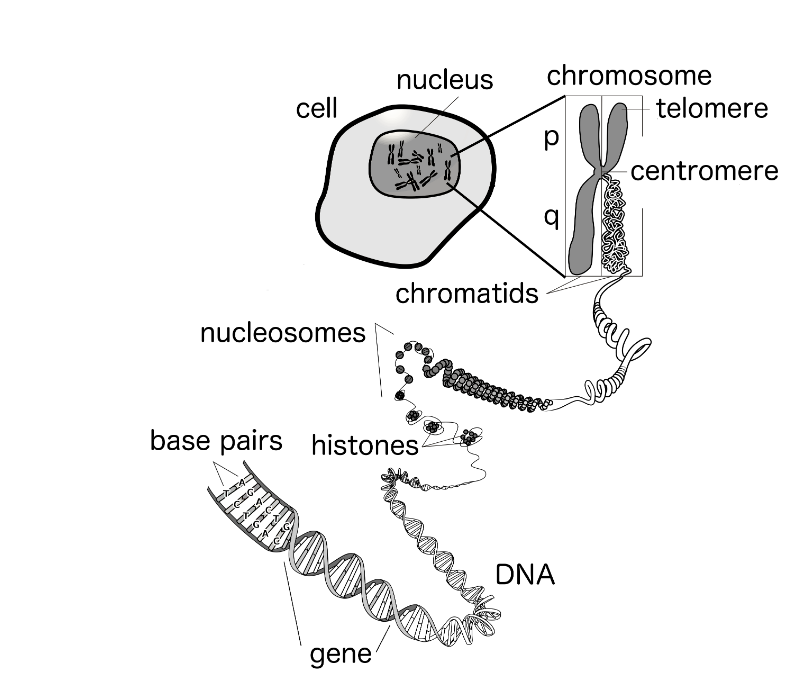
\includegraphics{images/genes_diagram.png}
\caption{An illustration of a chromosome, the DNA, and genes {[}R1{]}.}
\end{figure}

DNA is made up of bonds between base pairs of nucleotides. There are
four types of nucleotides found in DNA: adenine (A), cytosine (C),
guanine (G), and thymine (T); shown in the figure below.

\textit{Genes} are regions of the DNA which act as instructions to make
proteins. They also provide individuals with inherited characteristics.
The section with letters in the figure above shows an example gene.

\begin{figure}
\centering
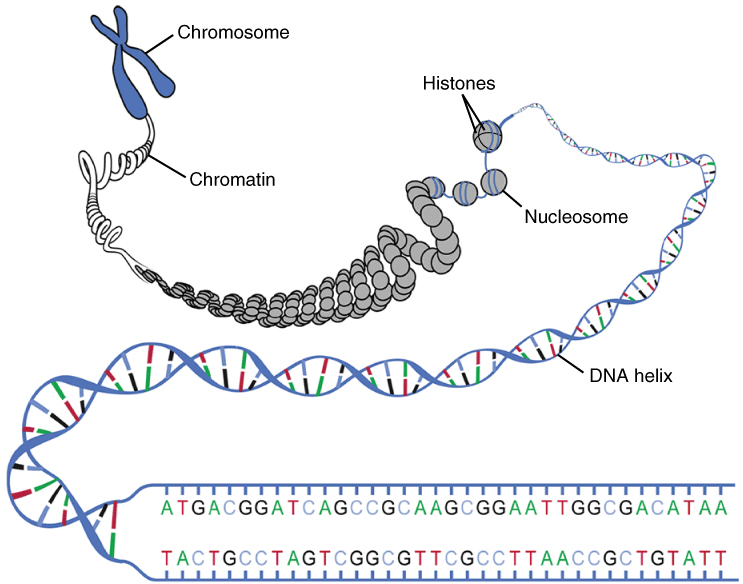
\includegraphics{images/nucleotides.jpg}
\caption{An illustration of nucleotides {[}R2{]}.}
\end{figure}

The bonds between the nucleotides hold the DNA strand together in the
form of a double helix. \textit{Single-nucleotide polymorphisms} (SNPs)
are common variations of the DNA observed in individuals; shown in the
figure below. They are variations of single nucleotides of the genome.

A \textit{locus} is a fixed position on a chromosome which contains a
gene {[}R3{]}. A DNA sequence at a locus can have different forms
(called alleles) from one copy of the chromosome to another. An
individual's genotype is their combination of alleles at a specific
locus.

\begin{figure}
\centering
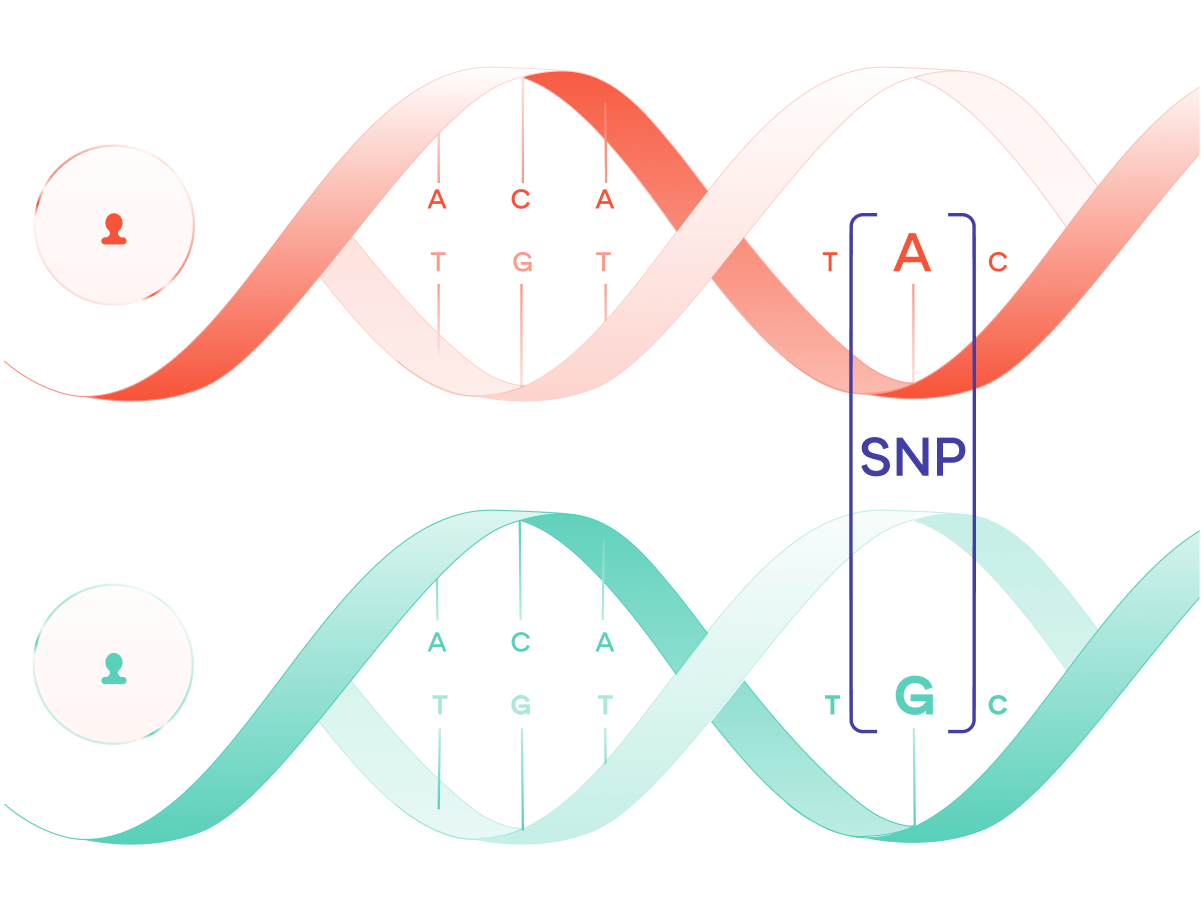
\includegraphics{images/snp.png}
\caption{An illustration of a SNP {[}R4{]}.}
\end{figure}

Let us consider the SNP shown in figure above with two alleles: A and G.
Hence, an individual has four possible genotypes that can be observed:
AA, AG, GA, and GG. The genotypes AA and GG are referred to as the
\textit{homozygous genotypes}. AG and GA are the
\textit{heterozygous genotypes}. The allele which is observed the least
in a sample population is termed the \textit{minor allele}.

The \textit{minor allele frequency} (MAF) is the rate at which the minor
allele occurs in a sample population.

The \textit{Hardy-Weinberg equilibrium} states that allele and genotype
rates are expected to remain the same in a population.

Finally, a \textit{phenotype} is an observable trait in an individual.
Examples include eye colour, hair colour, or a trait of a disease. There
is strong interest in discovering the relationships between genotype and
phenotype, as this can enable the attempted prediction of the risk of a
disease occurring in an individual, based on their genetic makeup. SNPs
are often tested for associations with phenotypes. The outcome variables
we use are (case-control) phenotype data.

\subsection{Downloading genetics data}\label{downloading-genetics-data}

First, we load a few useful packages:

\begin{Shaded}
\begin{Highlighting}[]
\FunctionTok{library}\NormalTok{(GEOquery)}
\FunctionTok{library}\NormalTok{(GSA)}
\end{Highlighting}
\end{Shaded}

To download the datasets, we can use the helpful \texttt{getGEO}
function from the \texttt{GEOquery} package loaded above. This function
is able to download a GEO object (which will contain the data needed for
fitting models) from the National Center for Biotechnology Information
(NCBI) database {[}L1{]}. The NCBI database contains many different
biomedical and genomic datasets. We are interested in the Gene
Expression Omnibus (GEO) datasets, which can be found through the search
function, although websites exist which have indexed the datasets
{[}L2{]}. In our example, we want to investigate whether we can predict
cases of inflammatory bowel diseases (Ulcerative colitis and Crohn's).
Searching the NCBI website for `Ulcerative colitis and Crohn's disease
comparison' yields the dataset {[}L3{]}. Using the dataset ID, we can
download the dataset using

\begin{Shaded}
\begin{Highlighting}[]
\NormalTok{gds1615 }\OtherTok{\textless{}{-}} \FunctionTok{getGEO}\NormalTok{(}\StringTok{\textquotesingle{}GDS1615\textquotesingle{}}\NormalTok{)}
\end{Highlighting}
\end{Shaded}

\subsection{Processing pipeline}\label{processing-pipeline}

Next, we need to process the data to prepare it for model fitting. We
are interested in obtaining three objects:

\begin{enumerate}
\def\labelenumi{\arabic{enumi}.}
\tightlist
\item
  The input data matrix, X. This will contain the gene expression data.
\item
  The response vector, y. This will contain the disease state of a
  patient (1 if the patient has an inflammatory bowel disease and 0
  otherwise).
\item
  The grouping structure indexes. This will contain group indexes for
  which groups (pathways) the genes belong to. This is only needed for
  the models which use grouping information (glasso and SGL).
\end{enumerate}

\subsection{Links}\label{links}

\begin{itemize}
\tightlist
\item
  {[}L1{]} \url{https://www.ncbi.nlm.nih.gov/gds}
\item
  {[}L2{]} \url{https://cola-gds.github.io/}
\item
  {[}L3{]}
  \url{https://www.ncbi.nlm.nih.gov/sites/GDSbrowser?acc=GDS1615}
\end{itemize}

\subsection{References}\label{references}

\begin{itemize}
\tightlist
\item
  {[}R1{]}
\end{itemize}

\end{document}
